\chapter*{Capítulo II}
\addtocontents{toc}{\protect\contentsline{chapter}{Capítulo II}{\thepage}{}}
\setcounter{chapter}{2} % Set the chapter counter to ensure proper numbering
\fancyhf{}
\rhead{Capítulo II}
\lhead{Informe de práctica Inicial en Air Logistics Corp.}
\fancyfoot[R]{\thepage} 

\section{Descripción de cargo}
El rol que le otorgó al estudiante fue el de practicante de ingeniería en el área de logística. A pesar de que se le asignaban tareas diversas en la empresa, los principales objetivos fueron los siguientes:
\begin{itemize}
    \item Migrar el sistema antiguo de inventario a un sistema más accesible y unificado para la organización.
    \item Migrar el sistema antiguo de generación de órdenes de trabajo a un sistema más accesible y unificado para la organización.
    \item Apoyar en la reestructuración del layout.
    \item Sistematizar el orden en los inventarios.
    \item Simplificar los procesos de la empresa, particularmente aquellos relacionados con las órdenes de trabajo.
    
     
\end{itemize}

\section{Actividades desarrolladas}
    \subsection{Creación de un ERP}
    A las puertas de una auditoría de la FAA, la empresa se encontraba en la necesidad de un sistema unificado y accesible en cualquier lugar del mundo para realizar varias de sus operaciones.
    
    \begin{figure}[H] % 'h' means "here", LaTeX tries to place it here
    \centering
    
\includegraphics[width=0.6\textwidth]{img/FAA.jpg} % Change to your image filename
    \caption{La FAA regula los talleres aeronáuticos panameños que trabajan con aeronaves estadounidenses.}
    \label{herr}
\end{figure}
    Por lo tanto, tras realizar una investigación, se reveló que una opción viable sería crear el sistema mediante un Framework de Python llamado \emph{Django}.
    
\begin{figure}[H] 
    \centering
    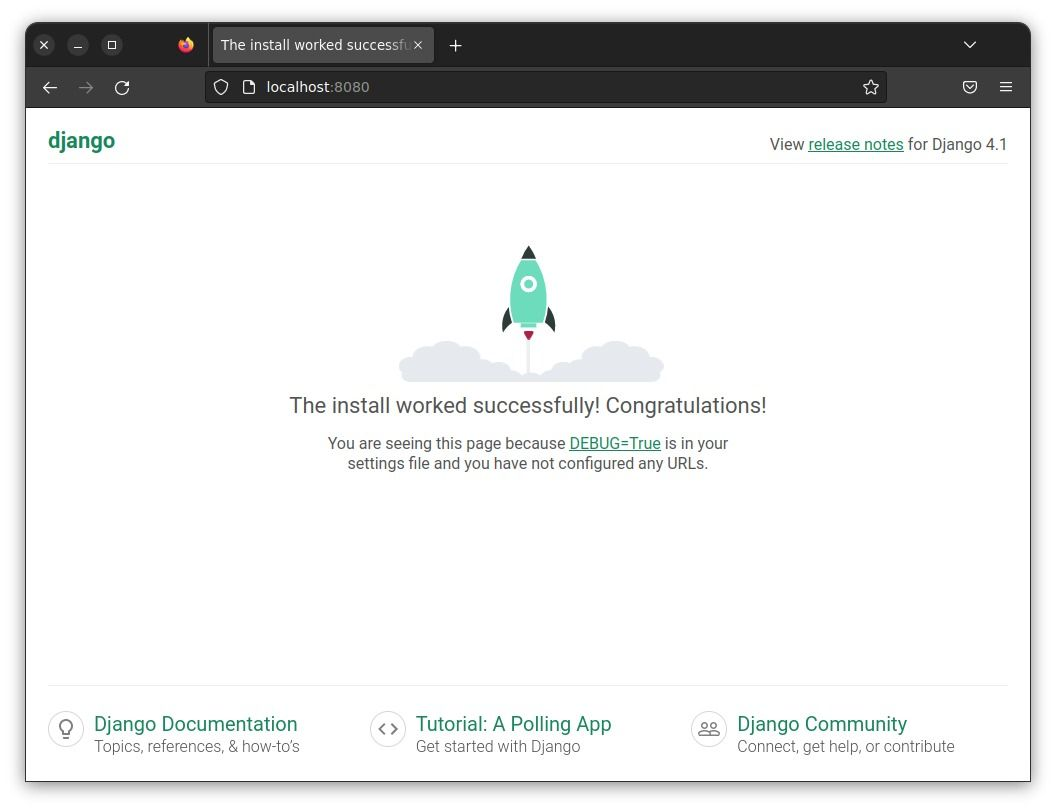
\includegraphics[width=0.5\textwidth]{img/djangostart4.jpg} % Change to your image filename
    \caption{La filosofía de Django es DRY y "con baterías incluidas". Evita volver a inventar la rueda.}
    \label{tools}
\end{figure}
    Django simplifica la creación de aplicaciones web, especialmente simplifica la creación y migraciones de bases de datos, solo se debe usar el lenguage de programación de python y no hay que realizar consultas de SQL necesariamente. Esto incrementa la seguridad también, pues este sistema es accesible vía internet.
     
    
\begin{figure}[H] % 'h' means "here", LaTeX tries to place it here
    \centering
    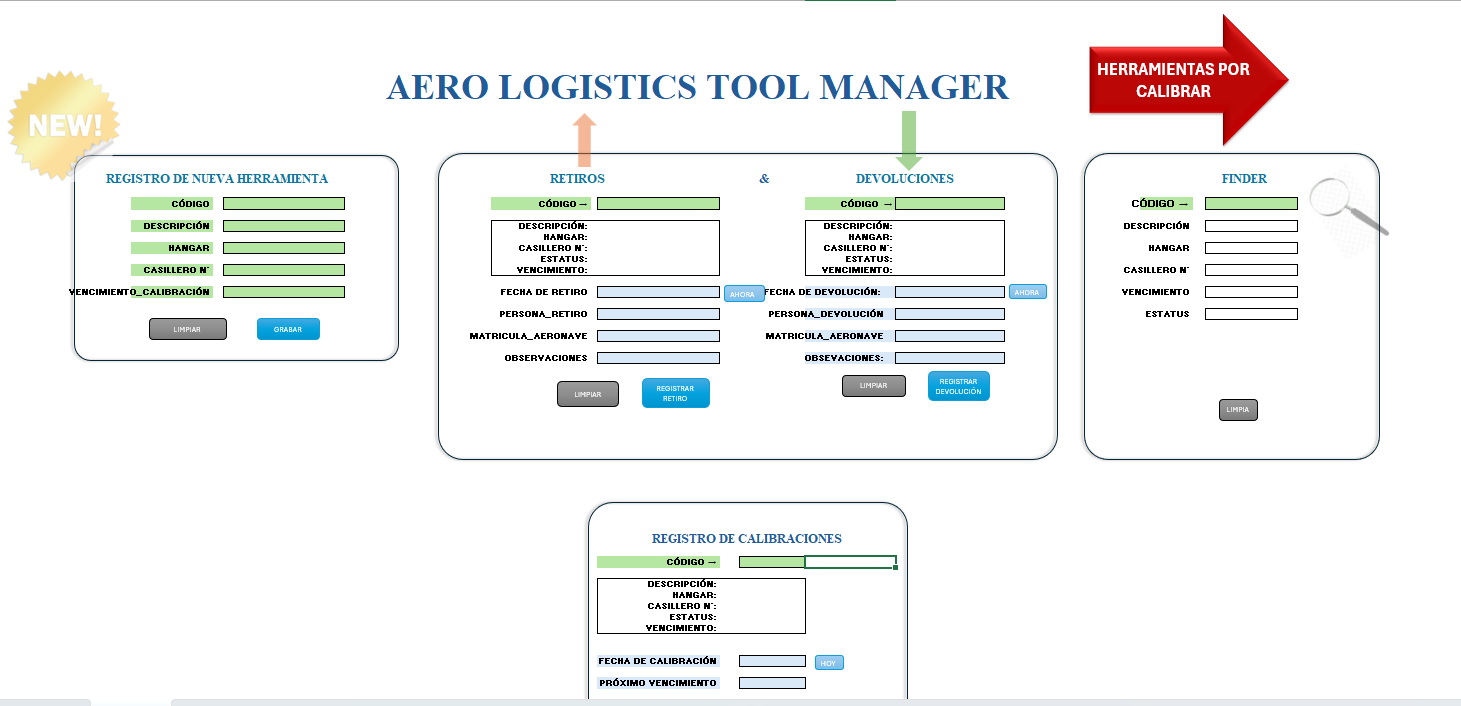
\includegraphics[width=1\textwidth]{Capitulos/tools.png} % Change to your image filename
    \caption{Formulario de ingreso para registro y movimientos de Herramientas calibradas.}
    \label{tools}
\end{figure}
    Finalmente tras muchas pruebas, se comprobó que el sistema era funcional. Se podía registrar cuándo, quién, dónde y mediante qué ordenador se retiró una pieza o herramienta. 
    
    \subsection{Automatización de los documentos generados en una Orden de Trabajo.}
    Se creo una macro en VBA que permitía la generación de múltiples documentos a partir de una solicitud de orden de trabajo. Los datos para generar estos documentos ya estaban incluidos en la solicitud. Por lo tanto, solo restaba almacenar los datos en variables y crear una lógica para reemplazarlos en las plantillas según el tipo de OT y según la nacionalidad de la aeronave.
\begin{figure}[h] % 'h' means "here", LaTeX tries to place it here
    \centering
    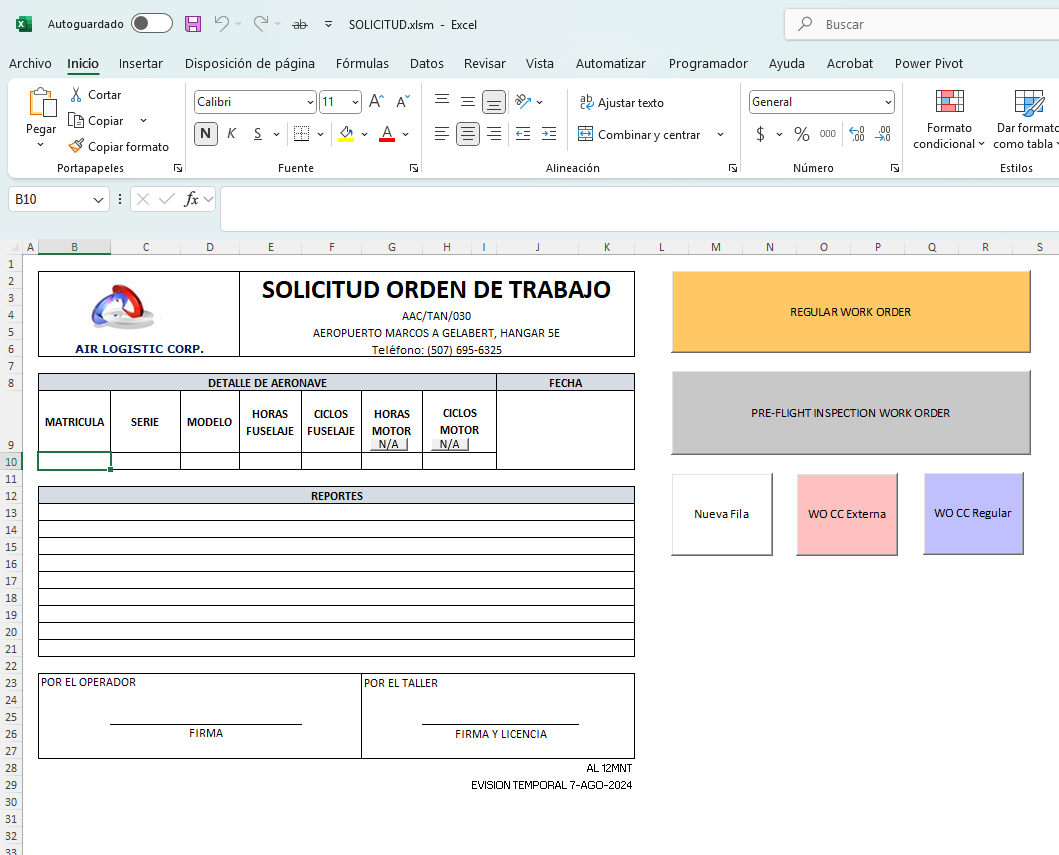
\includegraphics[width=0.6\textwidth]{Capitulos/workorder.png} % Change to your image filename
    \caption{Formulario de ingreso de solicitud de Orden de Trabajo}
    \label{workorder}
\end{figure}

    Los dos documentos principales en este proceso fueron la solicitud y el documento principal (Work Order/Pre-Flight Inspection). En caso de ser Work order se generaba n cantidad de Non-routine items, uno por cada reporte en la Work order.
    Todos estos documentos debían ser impresos y luego fusionados en un solo documento PDF. 

    Los non-routine items se imprimían a ambas caras.
    \subsection{Apoyo general en el hangar.}
    En algunas ocasiones, se le solicitaba al estudiante ayudar a movilizar piezas y demás objetos en el hangar. 
    \subsection{Apoyo en la verificación de checklist diarios.}
    A veces, se le solicitaba al estudiante realizar el checklist diario. El cual consistía de una revisión de ciertas partes del stock críticas para la seguridad de las aeronaves como para la seguridad de los hangares. Por ejemplo: revisión de la presión en tanques de $N_2$ y $O_2$; vigencia de los extintores y demás artículos de seguridad.
    \subsection{Transporte de objetos y documentos.}
    En raras ocasiones, se le encargaba al practicante transportar objetos dentro y fuera del aeropuerto. Ya sea documentos u objetos pesados. 
    

\section{Tecnologías empleadas}
\subsection{Python.}
Python es un lenguaje de programación multipropósito. Por lo que también se puede utilizar para desarrollar aplicaciones de escritorio. Aunque el desarrollo en Python se abandonó posteriormente, el aprendizaje de este lenguaje fue invaluable.
    \subsubsection{Tkinter.}
    Se trata de una librería de Python que permite desarrollar aplicaciones de escritorio sencillas. Sin embargo, la UI es muy anticuada. Da la impresión de ser del 2007.
    \subsubsection{PyQt5.}
    Permite hacer lo mismo que Tkinter pero con funciones más avanzadas y una UI mpas moderna. Sin embargo, la complejidad de esta librería aumenta signifcativamente si se compara con Tkinter. 
\subsection{MS Excel.}
Esta herramienta fue central en el desarrollo de todas las macros. Actuaba como un formulario de ingreso de datos, los que luego se utilizarían en el relleno automático de documentos e impresión posterior. Y, además, mediante VBA se pudo conectar al servidor de SQL para crear un sistema de inventario funcional y accesible a toda la red local.

\subsection{SQL Server.}
Este servidor fue funcamental para el sistema de inventario. Al habilitar su uso en la red fue posible que las personas tanto en las oficinas administrativas como los mecánicos en la parte inferior del hangar pudiesen realizar registros de piezas y herramientas sin necesidad de recorrer largas distancias.

\begin{figure}[h] % 'h' means "here", LaTeX tries to place it here
    \centering
    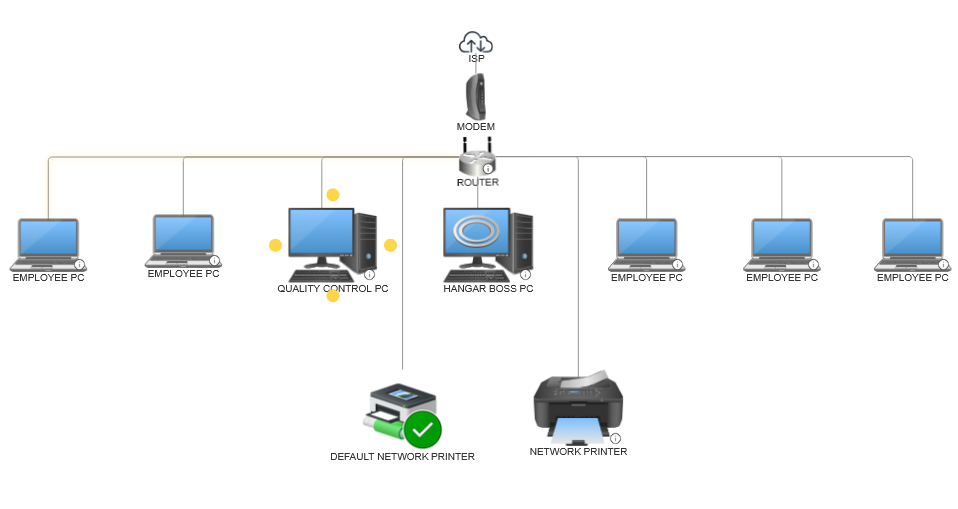
\includegraphics[width=0.6\textwidth]{prac/Network BEFORE.png} % Change to your image filename
    \caption{Red local antes de la implementación del servidor.}
    \label{Networkbef}
\end{figure}
En la figura \ref{after} se muestra la estructura de la red local final. De esta manera, debido a que el router tiene canal inalámbrico, es posible acceder a la base de datos desde cualquier lugar del hangar.
\begin{figure}[h] % 'h' means "here", LaTeX tries to place it here
    \centering
    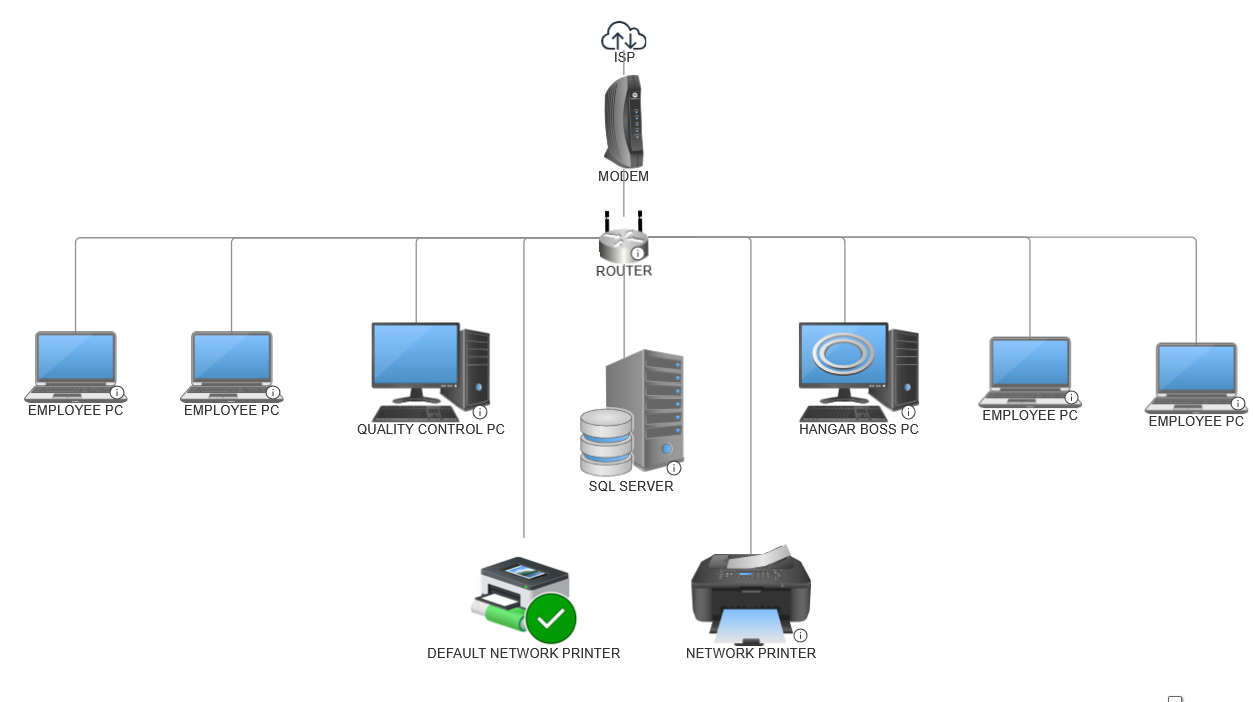
\includegraphics[width=0.6\textwidth]{prac/Network After.png} % Change to your image filename
    \caption{Red local antes de la implementación del servidor.}
    \label{after}
\end{figure}
\subsection{pdftk Server}
Aplicación que perimitía la manipulación de archivos PDF mediante cmd. Esto permitía manipular los PDF utilizando la automatización en VBA.
\section{Glosario}
\begin{itemize}
    \item Visual Basic for Applications (VBA): Es un lenguaje de programación de Microsoft diseñado para la automatización en el entorno de esta empresa, principalmente Office.
    \item Work Order: También conocida como Orden de Trabajo, es un documento generado cada vez que se le ha de realizar un mantenimiento a una aeronave. En este se llenan datos de la aeronave y del mantemimiento a realizar.
    \item Pre-flight inspection: Es un documento generado cada vez que una aeronave debe despegar. Incluye una lista de verificación de seguridad que debe ser llenada por el personal de tierra.
    \item FAA: Federal Aviation Administration. Es la agencia estadounidense que administra la aviación civil en su país.
    \item Non-routine Item: Documento que se genera por cada reporte realizado en la orden de trabajo (Work Order).
    
\end{itemize}